\chapter{Introduction} \label{cha:intro}

	In this Bachelor's Thesis a continuous-wave, frequency-modulated (CWFM) radar at 24 GHz is developed for real-time applications. There are situations where real-time acquisition of data is necessary, for instance, to obtain biomarkers such as heartbeat pulse variability and heartbeat or breathing patterns. The use of radar devices to monitor physiological signals is of great advantage, as it provides a means to do so without physical contact and therefore it provides more comfort to the patient \cite{Saner2020}. The remote monitoring of biomarkers and vital signs is of most importance in situations in which contact-based sensors cannot be used, such as treating patients with burnt skin, premature infants or performing sleep monitoring \cite{BoricLubecke2016}.  The current CWFM radar designs are based on a monolithic microwave integrated circuit (MMIC) with modifications and improvements to tailor the specific needs of each application.

	Several solutions that concentrate on obtaining such signals from radar systems have been developed at GMR-SSR to date. Radars operating in the W-band have been designed and characterised to measure biomarkers such as cardiopulmonary activity \cite{Antolinos2020} and other vital signs \cite{Sardinero2022}. More recent work is currently being developed to use these radars to extract gait patterns \cite{Zhang2012} and enable comparison between the gait of a healthy patient and a patient with Parkinson's disease \cite{Sardinero2022}.

	CWFM radars provide useful information from the signal they generate. For instance, the frequency of the signal obtained from beating the transmitted and received signals is proportional to the distance of the target from the antenna \cite[p.~20-27]{Richards2010}. Moreover, the frequency of the signal after beating the radar signals contains information on the position and movement of the target \cite{Wang2014}. Additionally, variations in the frequency of the radar signal carry information about the movement of the target \cite{Kernec2019,Gurbuz2019}.

	These signals must be digitised to extract the valuable information they contain. Current digitisation methods require expensive analogue-to-digital converters (ADCs) to process the samples from the signals \cite[p.~7]{Antolinos2020} \cite[p.~26]{Sardinero2022} and cannot provide real-time measurements \cite[p.~38]{Sardinero2022}. Besides, current systems that approach real-time often discard a large amount of useful samples.

	Thus, the design of a radar system with real-time data acquisition, processing, and transmission is developed for use in situations where real-time data of the radar and low-cost equipment are needed, such as performing gait analysis for Parkinson's disease characterisation.

	\section{Gait analysis in the context of Parkinson's disease} \label{sec:gait_analysis}

	Modern sensing technologies and approaches have shown promise in aiding the diagnosis and monitoring of symptoms in Parkinson's disease (PD) patients \cite{Biase2020}. Change in gait patterns is the most affected physical symptom related to a patient suffering from PD \cite{Zanardi2021}. The gait cycle of a walking person, either healthy or with a gait-affecting disease, can be measured and analysed quantitatively, such that relevant numerical data can be used to obtain an understanding on the level of PD severity in an unhealthy person \cite{Zanardi2021}.

	The gait cycle contains several spatiotemporal features which can be measured and observed to extract an objective conclusion on the broader gait analysis. The more commonly used types of features to describe the gait pattern of a person are shown in \cref{tab:gait_feat}. An illustration of the temporal distribution of these features on the gait cycle of a person is shown in \cref{fig:gait_drawing}. An image outlining the features of stride analysis is shown in \cref{fig:gait_stride}.

	{\footnotesize\renewcommand*{\arraystretch}{1.4}
		\begin{longtable}{@{}>{\raggedright\arraybackslash\bfseries}m{0.3\linewidth}>{\raggedright\arraybackslash}m{0.6\linewidth}@{}}
		\toprule
		Feature & Description \\* \midrule
		\endhead
		Gait cycle & Time from initial contact to the next initial contact on the same foot. It includes both the stance phase and swing phase.  \\
		Stance phase & Time during which the foot is in contact with the surface in a gait cycle. \\
		Swing phase & Time during which the foot is airborne in a gait cycle. \\
		Double limb support & Time during which both feet are in contact with the surface in a gait cycle. \\
		Single limb support & Time during which only one foot are in contact with the surface in a gait cycle. \\
		Step duration & Time period between two successive events of the same type on opposite limbs. \\
		Stride length & Linear distance on the surface between two successive initial contacts on the same limb. \\
		Step length & Linear distance on the surface between two successive events on the same limb. \\
		Step width & Horizontal linear distance between two points on opposite limbs. \\
		Foot progression angle & Angle between the longitudinal axis of the foot and the line of gait progression. \\* \bottomrule
		\caption[Spatiotemporal gait and stride features]{Spatiotemporal gait and stride features (adapted from \cite{Biase2020})}
		\label{tab:gait_feat}
	\end{longtable}}

	\begin{figure}[ht]
		\centering
		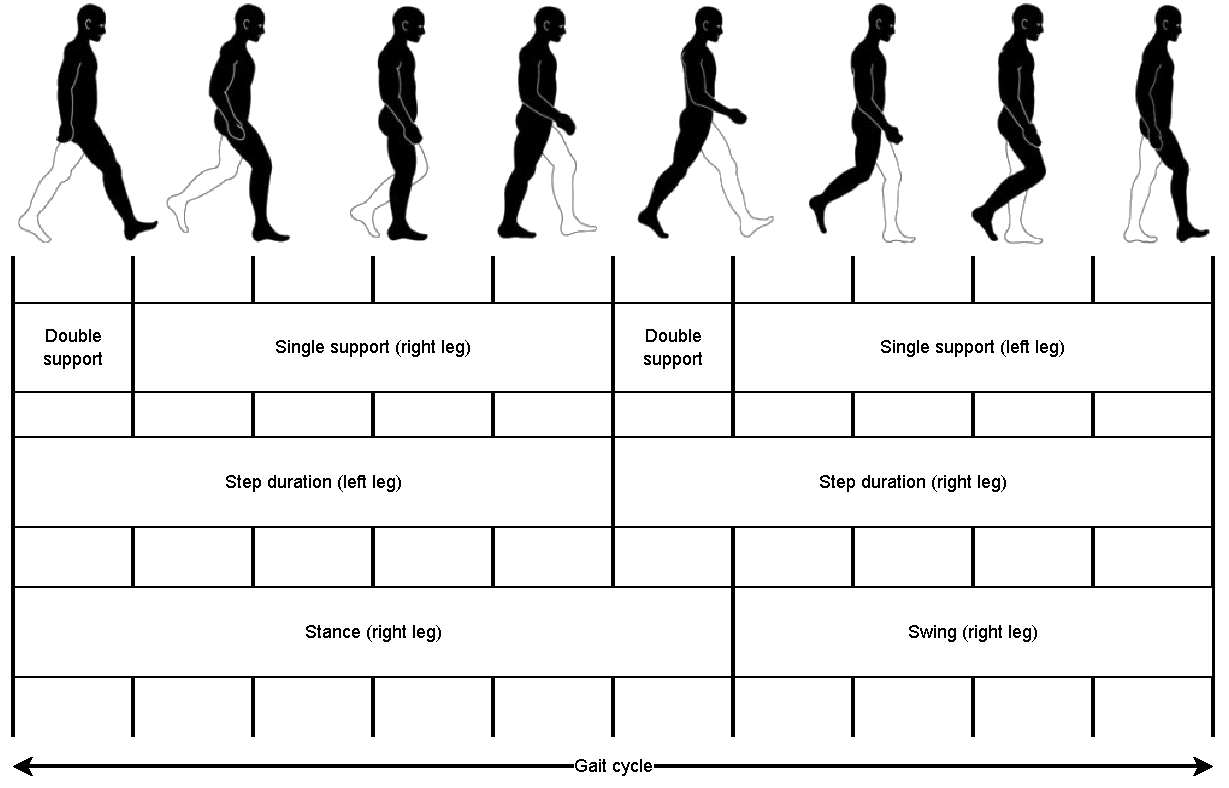
\includegraphics[width=\linewidth]{gait_cycle}
		\caption[Temporal characteristics of a human gait cycle]{Temporal characteristics of a human gait cycle (adapted from \cite{Zanardi2021})}
		\label{fig:gait_drawing}
	\end{figure}

    \begin{figure}[ht]
    	\centering
    	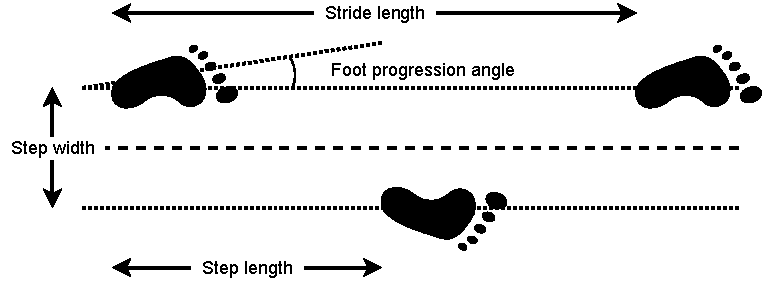
\includegraphics[width=0.8\linewidth]{gait_stride}
    	\caption[Spatial characteristics of a human gait cycle]{Spatial characteristics of a human gait cycle (adapted from \cite{Biase2020})}
    	\label{fig:gait_stride}
    \end{figure}

	These spatiotemporal features are related to position or velocity, such as the movement of the legs in the swing phase or the distance of other extremities to the body during the whole of the gait cycle \cite{Biase2020}. Therefore, a positional and velocity analysis can be carried out to quantise these movements using a variety of methodologies outlined in \cref{sec:gait_methods} ---of which radar sensing is the most promising---.

	\section{Overview of techniques used for gait analysis and measurement} \label{sec:gait_methods}
	\sectionmark{Overview of techniques for gait analysis and measurement}

	Parkinson's disease (PD) is of unknown aetiology and diagnostic certainty is impossible in life. The gold standard of diagnosis is via a neuropathological study. In clinical neuropathological studies, the success rate of diagnosis varies between 75-95\%, with accuracy varying depending on patient age, disease duration and medical specialist's experience.

	As discussed in \cref{sec:gait_analysis}, the diagnosis is prominently of clinical nature and it relies on the analysis of spatiotemporal motor biomarkers. The biometric quantification of these biomarkers is a current area of research and development. State-of-the-art advancements focus on the acquisition and quantisation of these motor biomarkers for developing computational models based on artificial intelligence (AI) technologies.

	These biometrics are performed through the obtention of data by making use of a diverse set of technologies, including the use of wearable sensors equipped with accelerometers and/or gyroscopes (or integrated inertial measurement units (IMU)), the use of infrared sensors, conventional video cameras, the analysis of handwriting or handwritten drawings using smart digitising tablets, or the interface with touch panels or devices \cite{Biase2020,Zanardi2021}. Ultimately, the aim is to enable the automatic characterisation of gait patterns \cite{Biase2020,Perumal2016}, postural and idle tremors \cite{Delrobaei2018}, kinetic tremors \cite{Rosenblum2013} or bradykinesia \cite{Mitsi2017}.

	Among the technologies listed, those based on accelerometers, gyroscopes and IMUs produce accurate results but suffer from limitations due to battery life, the need for additional hardware to store or transmit data, and the inconvenience of the individual carrying the devices \cite{Biase2020}. As a result, these technologies are deemed unsuitable for long periods of analysis and for non-obstructive monitoring. Alternatives based on multi-camera systems have been proposed \cite{MurodelaHerran2014} but they present limitations on low-light conditions and on environments with obstructing obstacles. Moreover, processing the data obtained is computationally expensive as they require algorithms based on computer vision (CV) and have limitations due to privacy concerns. In light of this, characterisation of handwritten media using smart tablet devices becomes a very good approximation \cite{Danna2019}, despite only allowing the characterisation of motor features of the upper extremities.

	In this context, new approaches based on the study of motor features by means of radar technologies have emerged. Radar systems allow for a non-invasive and contactless monitoring of motor features. Privacy concerns are no longer a limitation as radar technologies do not gather personally identifiable information such as images of the person. Radar signals do not rely on illumination constraints of the environment and thus work regardless of the light intensity levels. Moreover, radar systems are compact in size and low-cost and are not limited by obstacles as signal waves can travel past them. These benefits open the possibility on a paradigm shift in PD analysis and evaluation, as realisation of these technologies are based on the proven results of the analysis of movement patterns using continuous wave (CW) radars \cite{Antolinos2020, Seifert2019} by quantifying the micro-Doppler induced in the electromagnetic signal received.

	Therefore, radar systems are of great interest in the field of PD analysis through the characterisation of motor features including gait and tremor analysis.
	
	
	\section{Vital signs monitoring}
	
	Vital signs monitoring gives important information about the overall health of a patient. They comprise medical information such as heart rate pulse, respiration patterns or blood oxygenation levels \cite{Iyer2022}. Moreover, the continuous monitoring and analysis of these signs has been deemed important for the supervision of symptoms due to illnesses in patients undergoing observation or treatments \cite{Prgomet2016,Weenk2017,Villarroel2014}.
	
	Heart rate variability (HRV) is currently monitored using various methods such as electrocardiography (ECG) electrodes, pulse oximeters, photoplethysmography (PPG), and wearable devices like inertial movement units (IMU) \cite{Antolinos2020, Lv2018}. Breathing rate is often measured manually with a timer or using oronasal sensors that detect changes in air pressure caused by respiration. These traditional methods can be inaccurate due to random body movements (RBM) and can be uncomfortable for users, especially during ambulatory monitoring \cite{Antolinos2020}.
	
	Radar-based solutions have been proposed as an alternative for non-contact measurement of heart rate and respiration rate. Continuous-wave frequency modulated radars (CWFM), in particular, offer several advantages such as the ability to work at higher frequencies and detect smaller movements in the centimetre to millimetre range \cite{Lv2018}. CWFM radars work on the movement of organs and tissues, providing measurements on displacement velocity and position. By analysing the signal received by the radar, it is possible to identify characteristics related to heart rate pulse and breathing patterns \cite{Antolinos2020}.
	
	Another way that millimetre-wave radar can be used to monitor vital signs is by measuring the absorption of the radar waves by the body. Different tissues and organs absorb the radar waves at different rates, which can be used to measure things like blood flow and oxygen saturation \cite{Weenk2017}.
	
	For instance, the absorption of millimetre-wave radar by the blood can be used to measure blood flow in different parts of the body. The absorption of millimetre-wave radar by the tissue can also be used to measure the oxygen saturation of the tissue, which can be an indicator of the overall health of the tissue \cite{Amin2017, Antolinos2020}
	
	These technologies are based on the successful use of continuous wave (CW) radars to analyse movement patterns by quantifying the micro-Doppler effect on the electromagnetic signal received \cite{Antolinos2020, Seifert2019}. 
	
	Therefore, radar systems are also of great interest in the field of vital signs monitoring and analysis due to their ability to characterize the movement properties of organs and tissues in the human body, which can be useful in understanding and analysing heart rate and breathing patterns.
	
\section{Challenges of current applications of CW radars for gait analysis and vital signs monitoring}

\section{Objectives}

	The main objective of this Bachelor's Thesis is to develop a radar sensor that enables digitisation of the radar signals and allows the extraction of biomarkers, such as vital signs and gait patterns. The radar sensor is based on the W-band CWFM radar (whose designs are  outlined in \cite{Sardinero2022} and \cite{Montesano2019}). It is of interest that these sensors can provide real-time measurements while being low-cost. The secondary objectives for this project as well as the means to fulfil them are as follows:
	\begin{itemize}
		\item \textbf{Characterisation and modification of a 24 GHz radar module based on a commercial MMIC}. A currently designed and operational radar sensor module will be modified and adapted to create a CWFM radar module suitable for the outlined applications. Some modifications to the processing PCB will be carried out.
		\item \textbf{Study and characterisation of the intermediate frequency (IF) signals generated by the radar module}. The IF signals output from the radar will be measured in amplitude and frequency. The useful information carried in the signals will be analysed and discussed.
		\item \textbf{Selection of a microprocessor unit (MCU) for data processing and transmission.} An appropriate MCU will be selected according to the needs and specifications of the system, which include low cost and support for a wireless transmission protocol. This MCU will sample and process the radar signals.
		\item \textbf{Design of an IF stage to condition the signals for the MCU}. The IF signals must be conditioned before being supplied to the MCU. For this purpose, a filtering and conditioning stage is to be designed, manufactured and measured.
		\item \textbf{Development of the data processing algorithm and system}. The IF signals data must be processed before being transmitted to the receiving device. For that matter, a digital processing stage will be designed and implemented and its performance will be measured.
		\item \textbf{Design of a transmission pipeline using Bluetooth Low Energy (BLE)}. After study and consideration of other wireless technologies, a data transmission pipeline based on BLE will be designed and implemented to transmit the information contained in the processed radar signals.
		\item \textbf{Design of a user application for monitoring radar signals in real-time}. A GUI application is developed for a receiving device to enable reception, visualisation and storage of the received signals.
		\item \textbf{Integration of all objectives to form a complete radar system}. The complete system performance and its limitations will be analysed and measured.
	\end{itemize}

	This Bachelor Thesis is structured as follows. The basic working principle of CWFM radars will be introduced in this chapter. In Chapter 2 the characterisation and modification of a 24 GHz radar module is carried out and a suitable MCU is selected, which must meet some criteria. In Chapter 3 it is designed an IF stage to condition the radar signals for the MCU sampling capabilities and its performance is simulated using circuit simulation software and tested experimentally. In Chapter 4 digital signal processing techniques are applied to process the radar signals and extract useful information limiting the number of necessary samples to transmit. It is also designed a transmission pipeline using BLE to send the radar information to the receiving end. In Chapter 6 a user application is developed to receive, store and visualise the processed radar signals. It is implemented in a PC and with a graphical user interface. Finally, in Chapter 7, the complete system is formed by integrating all parts and it is characterised experimentally and its performance is measured, establishing working limitations and laying out future improvements.